Recent years have featured a trend towards pre-trained language representations in NLP systems, applied in increasingly flexible and task-agnostic ways for downstream transfer.  First, single-layer representations were learned using word vectors \cite{mikolov2013efficient, pennington2014glove} and fed to task-specific architectures, then RNNs with multiple layers of representations and contextual state were used to form stronger representations \cite{dai2015semi, mccann2017learned, peters2018dissecting} (though still applied to task-specific architectures), and more recently pre-trained recurrent or transformer language models \cite{vaswani2017attention}  have been directly fine-tuned, entirely removing the need for task-specific architectures \cite{radford2018gpt1, devlin2018bert, howard2018universal}.

\begin{figure}[b!]
\centering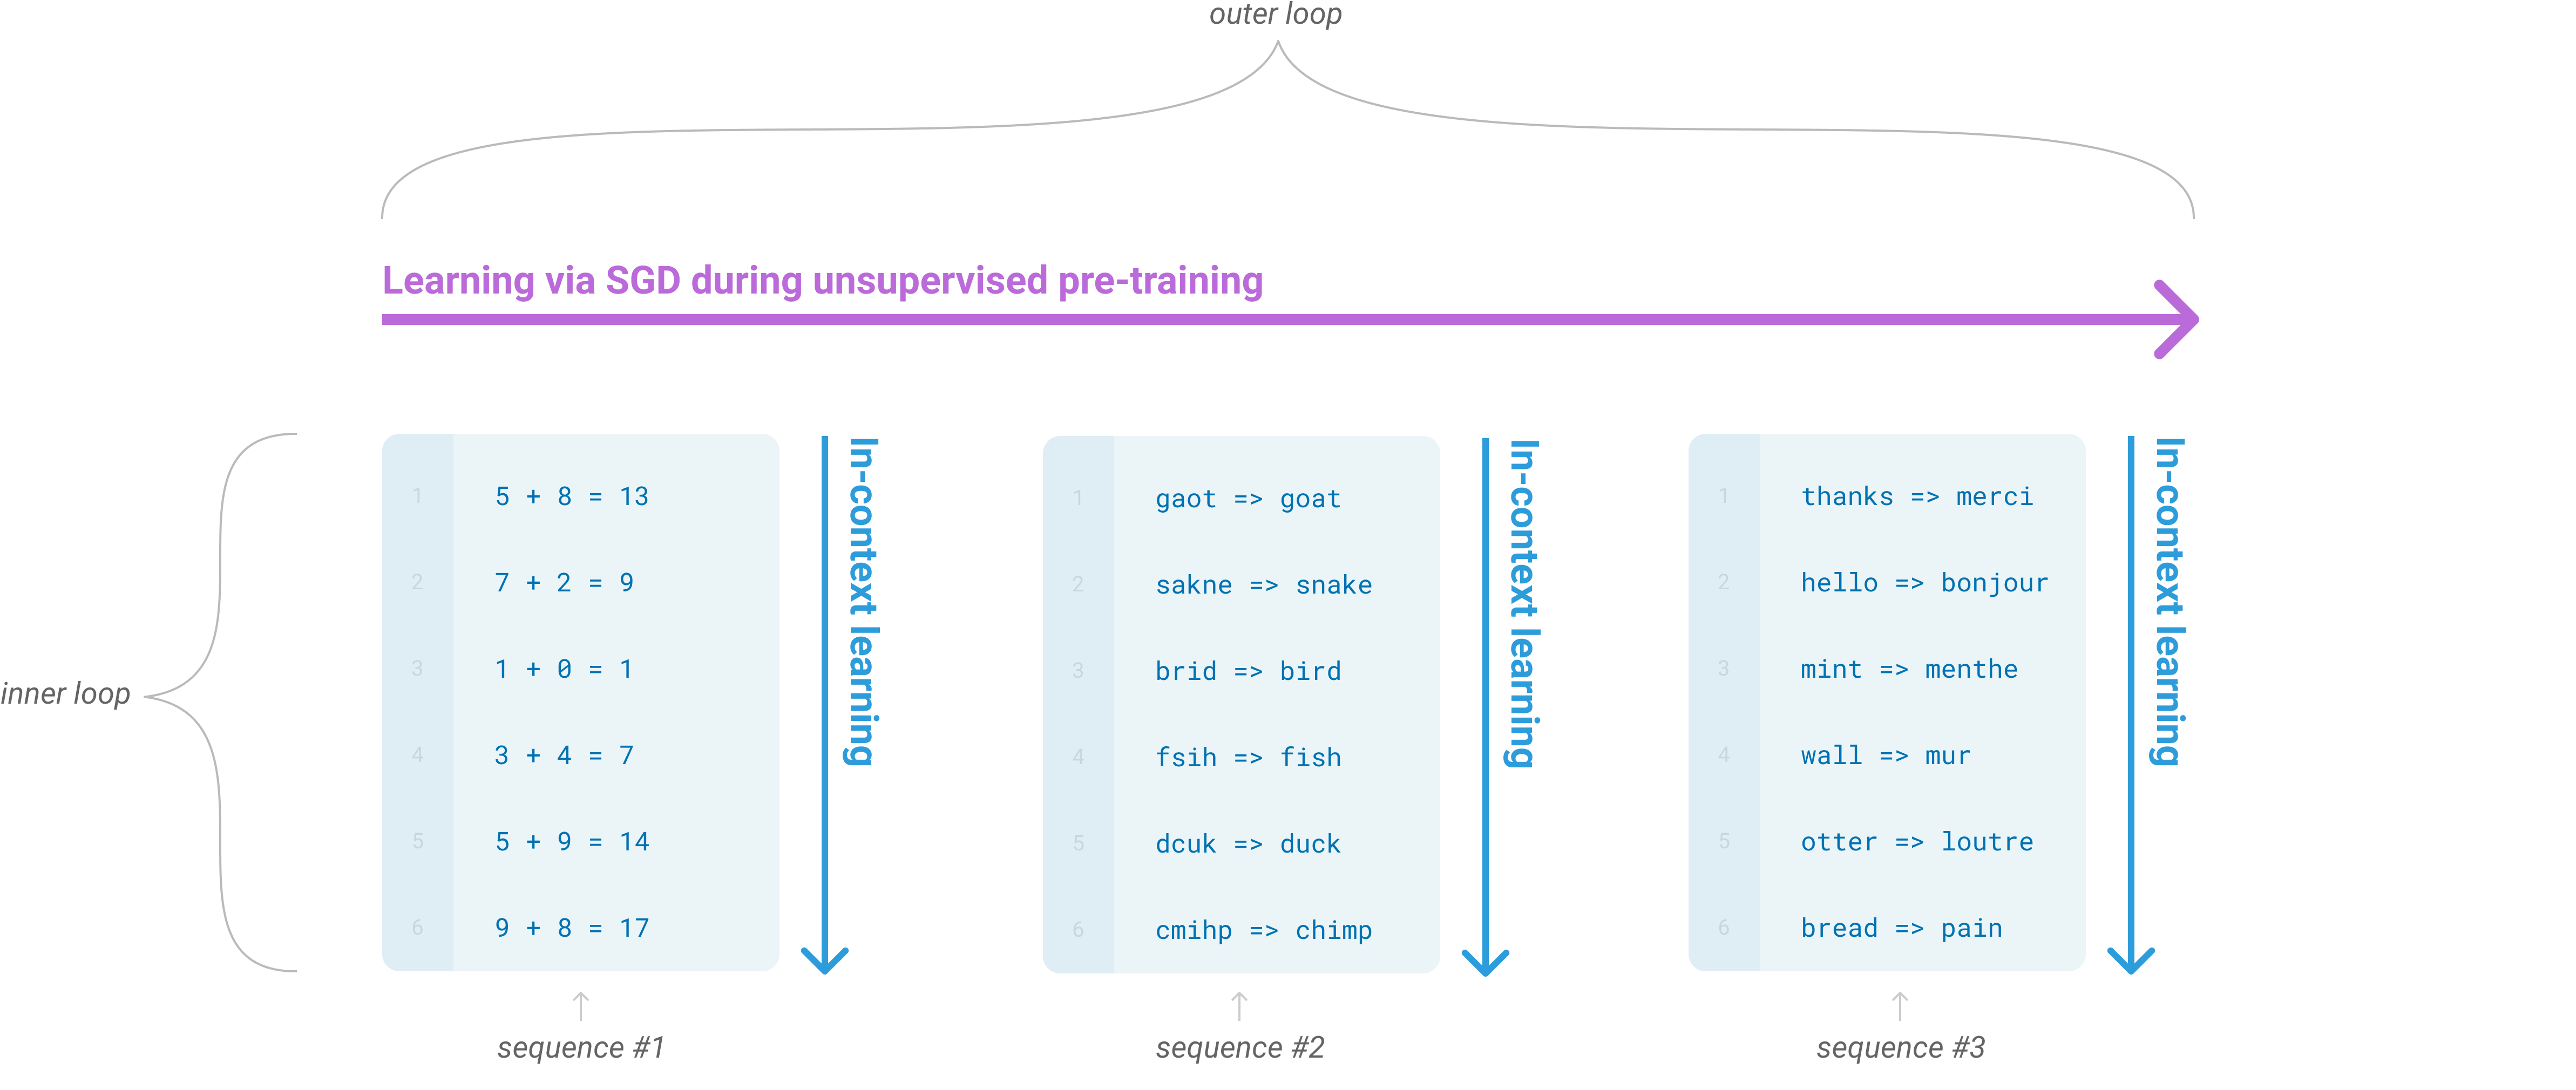
\includegraphics[width=1.0\linewidth]{figures/metalearning.png}
\caption{\textbf{Language model meta-learning.} During unsupervised pre-training, a language model develops a broad set of skills and pattern recognition abilities. It then uses these abilities at inference time to rapidly adapt to or recognize the desired task. We use the term ``in-context learning" to describe the inner loop of this process, which occurs within the forward-pass upon each sequence. The sequences in this diagram are not intended to be representative of the data a model would see during pre-training, but are intended to show that there are sometimes repeated sub-tasks embedded within a single sequence.
}
\label{figure:metalearning}
\end{figure}

This last paradigm has led to substantial progress on many challenging NLP tasks such as reading comprehension, question answering, textual entailment, and many others, and has continued to advance based on new architectures and algorithms \cite{raffel2019t5, liu2019roberta, yang2019xlnet, lan2019albert}. However, a major limitation to this approach is that while the architecture is task-agnostic, there is still a need for task-specific datasets and task-specific fine-tuning: to achieve strong performance on a desired task typically requires fine-tuning on a dataset of thousands to hundreds of thousands of examples specific to that task.  Removing this limitation would be desirable, for several reasons.

First, from a practical perspective, the need for a large dataset of labeled examples for every new task limits the applicability of language models.  There exists a very wide range of possible useful language tasks, encompassing anything from correcting grammar, to generating examples of an abstract concept, to critiquing a short story.  For many of these tasks it is difficult to collect a large supervised training dataset, especially when the process must be repeated for every new task.

Second, the potential to exploit spurious correlations in training data fundamentally grows with the expressiveness of the model and the narrowness of the training distribution. This can create problems for the pre-training plus fine-tuning paradigm, where models are designed to be large to absorb information during pre-training, but are then fine-tuned on very narrow task distributions. For instance \cite{hendrycks2020pretrained} observe that larger models do not necessarily generalize better out-of-distribution. There is evidence that suggests that the generalization achieved under this paradigm can be poor because the model is overly specific to the training distribution and does not generalize well outside it \cite{yogatama2019learning, mccoy2019right}. Thus, the performance of fine-tuned models on specific benchmarks, even when it is nominally at human-level, may exaggerate actual performance on the underlying task \cite{gururangan2018annotation, niven2019probing}.

Third, humans do not require large supervised datasets to learn most language tasks -- a brief directive in natural language (e.g. ``please tell me if this sentence describes something happy or something sad'') or at most a tiny number of demonstrations (e.g. ``here are two examples of people acting brave; please give a third example of bravery'') is often sufficient to enable a human to perform a new task to at least a reasonable degree of competence.  Aside from pointing to a conceptual limitation in our current NLP techniques, this adaptability has practical advantages -- it allows humans to seamlessly mix together or switch between many tasks and skills, for example performing addition during a lengthy dialogue.  To be broadly useful, we would someday like our NLP systems to have this same fluidity and generality.

One potential route towards addressing these issues is meta-learning\footnote{In the context of language models this has sometimes been called ``zero-shot transfer'', but this term is potentially ambiguous: the method is ``zero-shot'' in the sense that no gradient updates are performed, but it often involves providing inference-time demonstrations to the model, so is not truly learning from zero examples.  To avoid this confusion, we use the term ``meta-learning'' to capture the inner-loop / outer-loop structure of the general method, and the term ``in context-learning" to refer to the inner loop of meta-learning. We further specialize the description to ``zero-shot", ``one-shot", or ``few-shot" depending on how many demonstrations are provided at inference time.  These terms are intended to remain agnostic on the question of whether the model learns new tasks from scratch at inference time or simply recognizes patterns seen during training -- this is an important issue which we discuss later in the paper, but ``meta-learning'' is intended to encompass both possibilities, and simply describes the inner-outer loop structure.} -- which in the context of language models means the model develops a broad set of skills and pattern recognition abilities at training time, and then uses those abilities at inference time to rapidly adapt to or recognize the desired task (illustrated in Figure \ref{figure:metalearning}). Recent work \cite{radford2019language} attempts to do this via what we call ``in-context learning", using the text input of a pretrained language model as a form of task specification: the model is conditioned on a natural language instruction and/or a few demonstrations of the task and is then expected to complete further instances of the task simply by predicting what comes next.


While it has shown some initial promise, this approach still achieves results far inferior to fine-tuning -- for example \cite{radford2019language} achieves only 4\% on Natural Questions, and even its 55 F1 CoQa result is now more than 35 points behind the state of the art.  Meta-learning clearly requires substantial improvement in order to be viable as a practical method of solving language tasks.

Another recent trend in language modeling may offer a way forward.  In recent years the capacity of transformer language models has increased substantially, from 100 million parameters \cite{radford2018gpt1}, to 300 million parameters \cite{devlin2018bert}, to 1.5 billion parameters \cite{radford2019language}, to 8 billion parameters \cite{shoeybi2019megatronlm}, 11 billion parameters \cite{raffel2019t5}, and finally 17 billion parameters \cite{turing_17m}.  Each increase has brought improvements in text synthesis and/or downstream NLP tasks, and there is evidence suggesting that log loss, which correlates well with many downstream tasks, follows a smooth trend of improvement with scale \cite{kaplan2020scaling}.  Since in-context learning involves absorbing many skills and tasks within the parameters of the model, it is plausible that in-context learning abilities might show similarly strong gains with scale.


\begin{figure}
\centering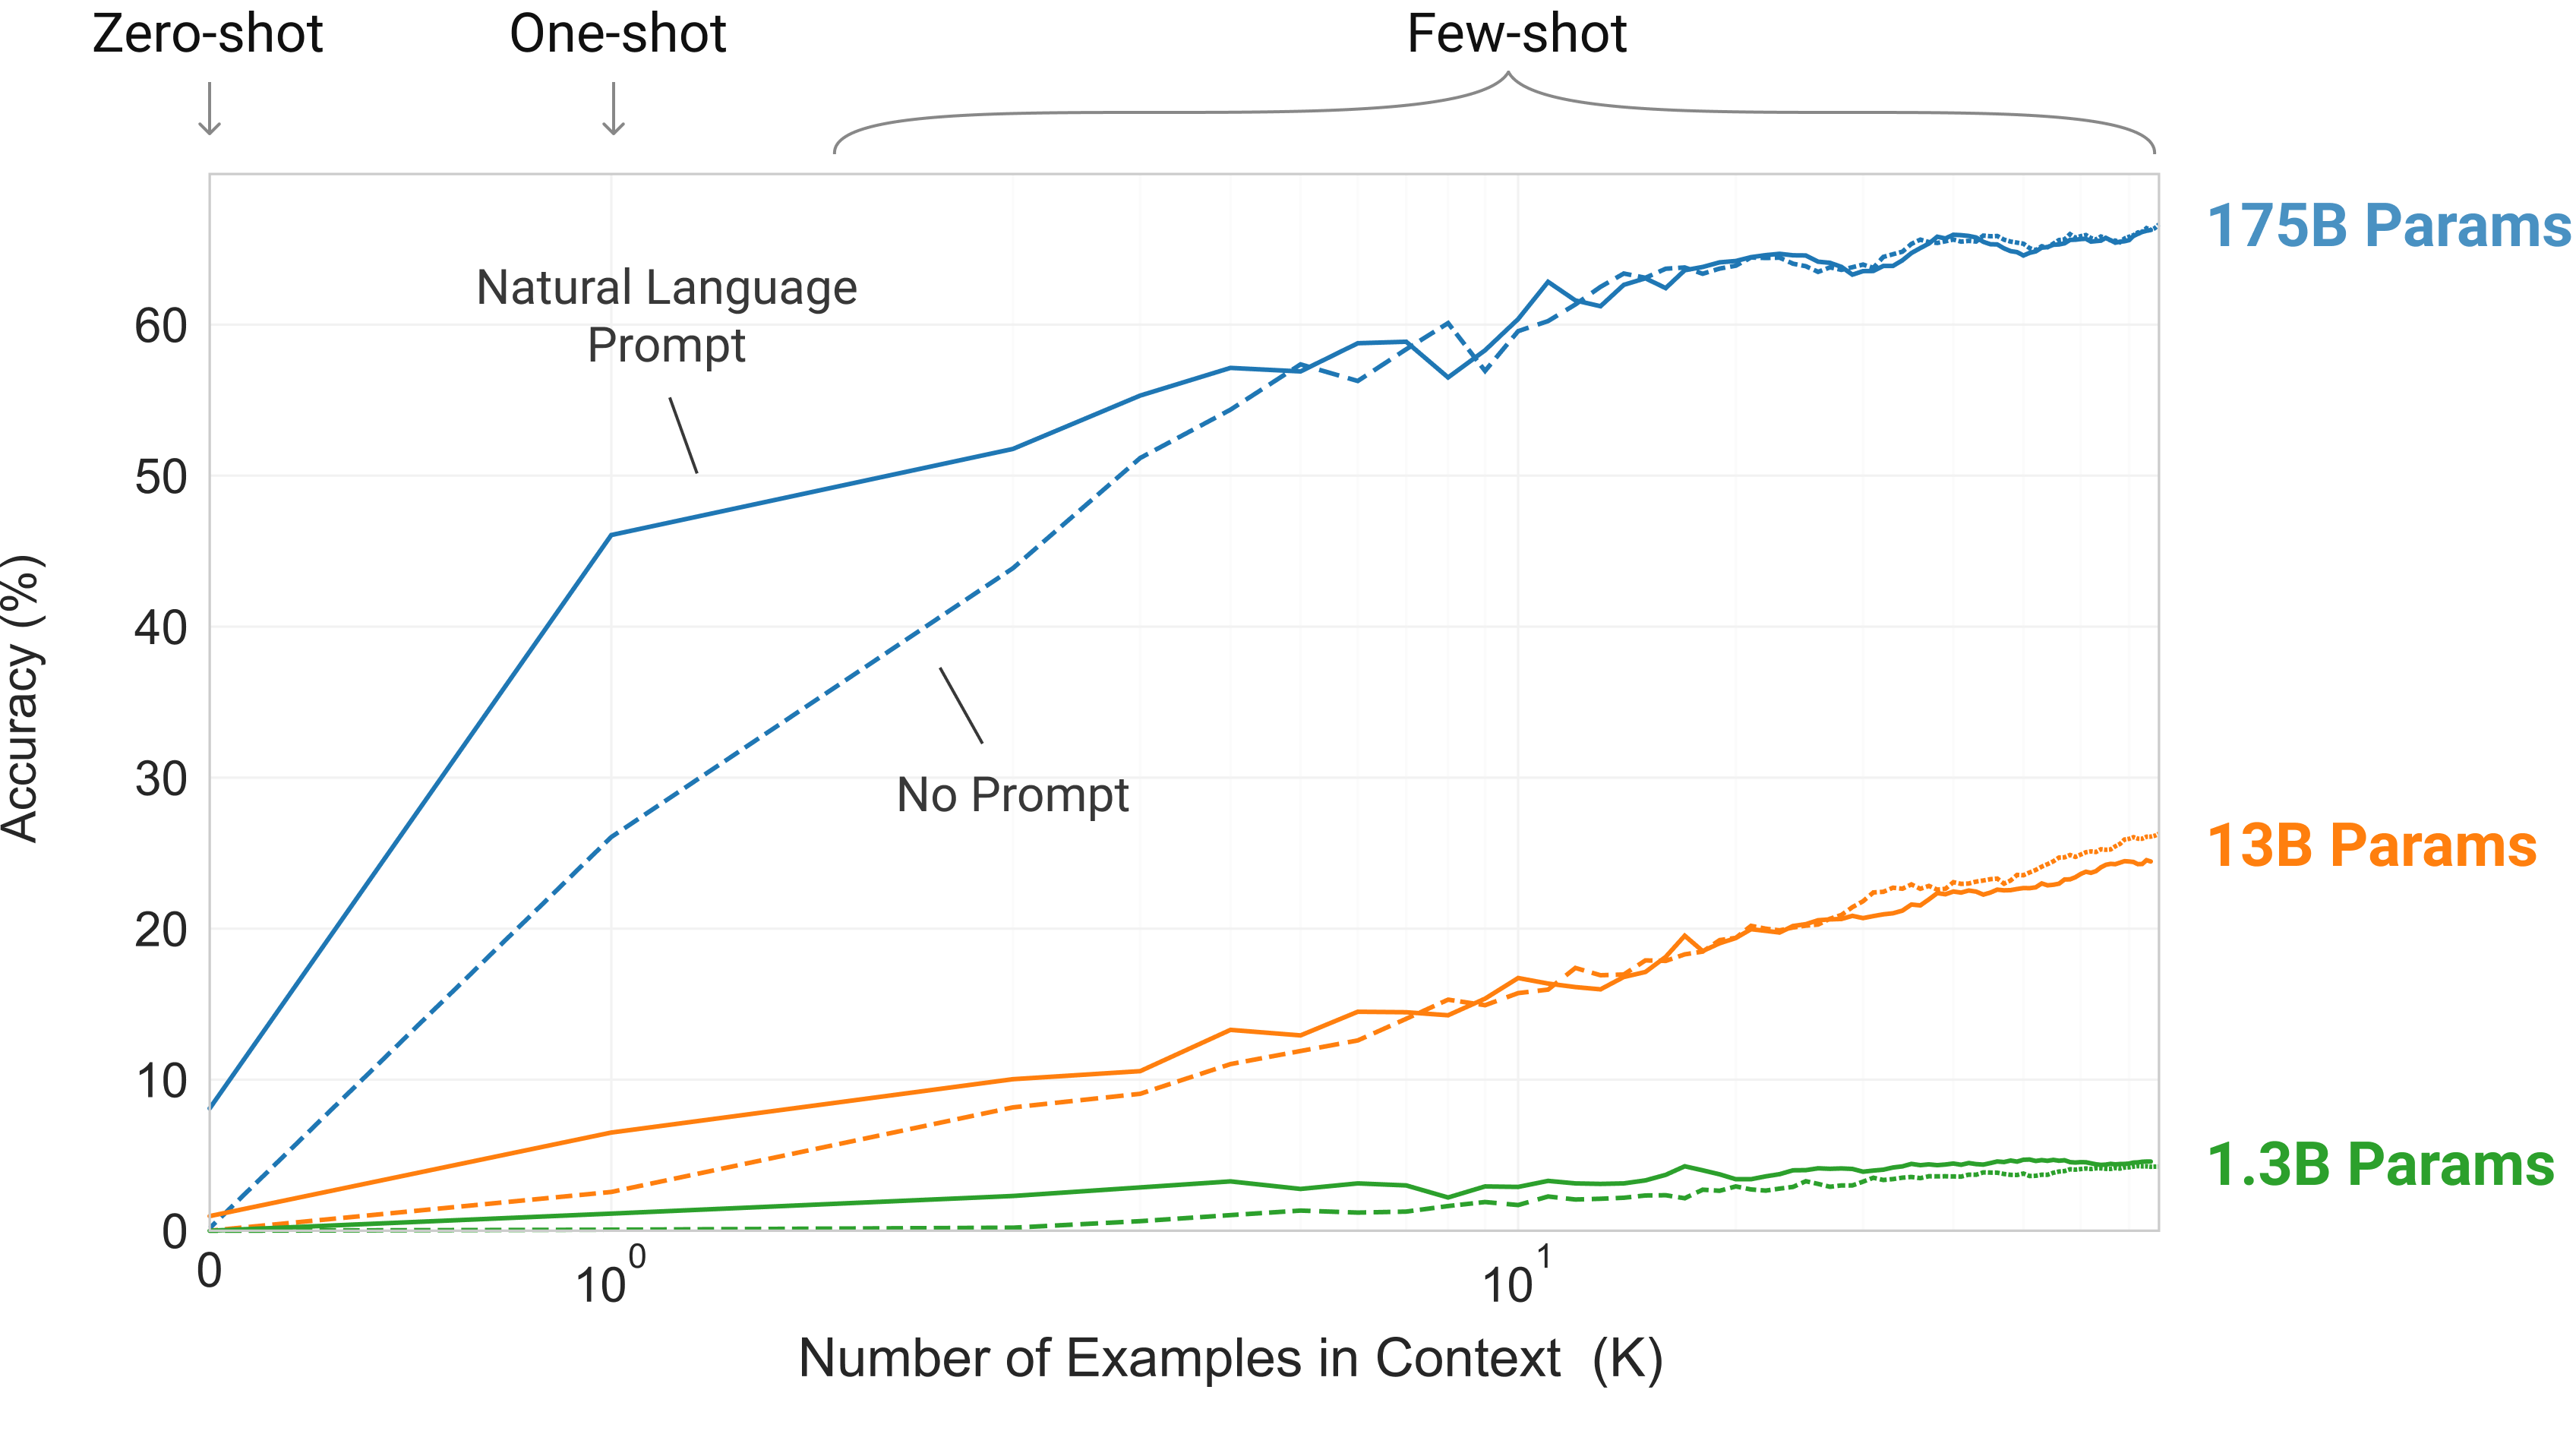
\includegraphics[width=0.8\linewidth]{graphs/img/in_context_learning.png}
\caption{\textbf{Larger models make increasingly efficient use of in-context information.}~~~We show in-context learning performance on a simple task requiring the model to remove random symbols from a word, both with and without a natural language task description (see Sec. \ref{section:Word_Scrambling_and_Manipulation_Tasks}). The steeper ``in-context learning curves'' for large models demonstrate improved ability to learn a task from contextual information. We see qualitatively similar behavior across a wide range of tasks.}
\label{graph:scramble_prompted}
\end{figure}

\begin{figure}
\begin{center}
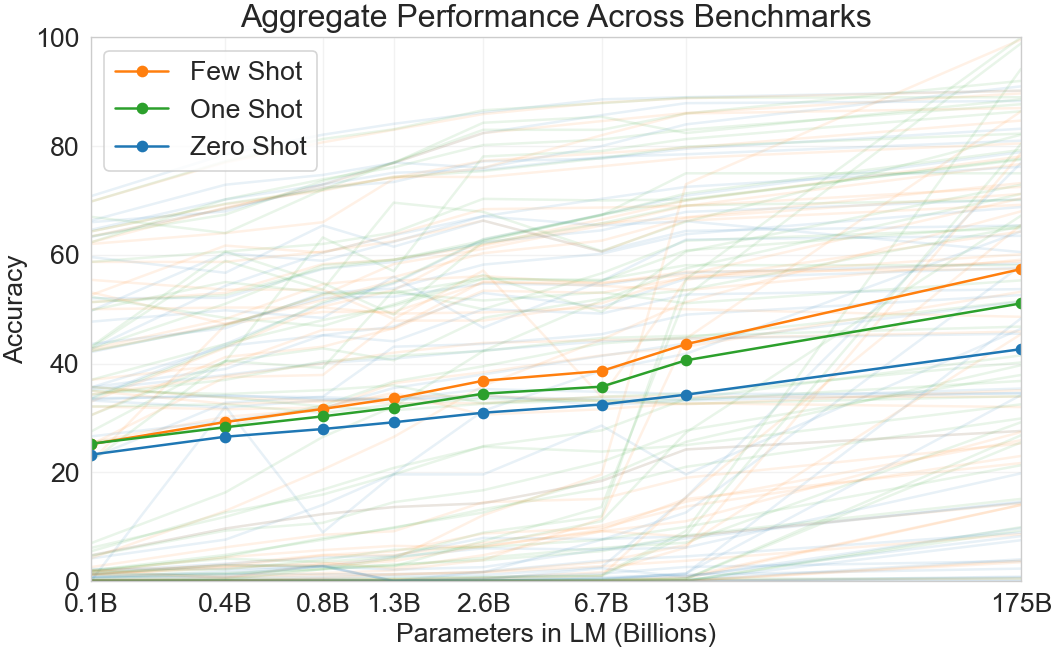
\includegraphics[width=0.7\linewidth]{graphs/aggregate_performance.png}
\end{center}
\caption{\textbf{Aggregate performance for all 42 accuracy-denominated benchmarks}~~~While zero-shot performance improves steadily with model size, few-shot performance increases more rapidly, demonstrating that larger models are more proficient at in-context learning. See Figure \ref{graph:superglue_analysis} for a more detailed analysis on SuperGLUE, a standard NLP benchmark suite.}
\label{figure:aggregate_performance}
\end{figure}

In this paper, we test this hypothesis by training a 175 billion parameter autoregressive language model, which we call GPT-3, and measuring its in-context learning abilities.  Specifically, we evaluate GPT-3 on over two dozen NLP datasets, as well as several novel tasks designed to test rapid adaptation to tasks unlikely to be directly contained in the training set.  For each task, we evaluate GPT-3 under 3 conditions: (a) ``few-shot learning'', or in-context learning where we allow as many demonstrations as will fit into the model’s context window (typically 10 to 100), (b) ``one-shot learning'', where we allow only one demonstration, and (c) ``zero-shot'' learning, where no demonstrations are allowed and only an instruction in natural language is given to the model.  GPT-3 could also in principle be evaluated in the traditional fine-tuning setting, but we leave this to future work.

 Figure \ref{graph:scramble_prompted} illustrates the conditions we study, and shows few-shot learning of a simple task requiring the model to remove extraneous symbols from a word. Model performance improves with the addition of a natural language task description, and with the number of examples in the model's context, $K$. Few-shot learning also improves dramatically with model size.  Though the results in this case are particularly striking, the general trends with both model size and number of examples in-context hold for most tasks we study.  We emphasize that these ``learning'' curves involve no gradient updates or fine-tuning, just increasing numbers of demonstrations given as conditioning.

Broadly, on NLP tasks GPT-3 achieves promising results in the zero-shot and one-shot settings, and in the the few-shot setting is sometimes competitive with or even occasionally surpasses state-of-the-art (despite state-of-the-art being held by fine-tuned models).  For example, GPT-3 achieves 81.5 F1 on CoQA in the zero-shot setting, 84.0 F1 on CoQA in the one-shot setting, 85.0 F1 in the few-shot setting.  Similarly, GPT-3 achieves 64.3\% accuracy on TriviaQA in the zero-shot setting, 68.0\% in the one-shot setting, and 71.2\% in the few-shot setting, the last of which is state-of-the-art relative to fine-tuned models operating in the same closed-book setting.

GPT-3 also displays one-shot and few-shot proficiency at tasks designed to test rapid adaption or on-the-fly reasoning, which include unscrambling words, performing arithmetic, and using novel words in a sentence after seeing them defined only once.  We also show that in the few-shot setting, GPT-3 can generate synthetic news articles which human evaluators have difficulty distinguishing from human-generated articles.

At the same time, we also find some tasks on which few-shot performance struggles, even at the scale of GPT-3.  This includes natural language inference tasks like the ANLI dataset, and some reading comprehension datasets like RACE or QuAC.  By presenting a broad characterization of GPT-3's strengths and weaknesses, including these limitations, we hope to stimulate study of few-shot learning in language models and draw attention to where progress is most needed.  

A heuristic sense of the overall results can be seen in Figure \ref{figure:aggregate_performance}, which aggregates the various tasks (though it should not be seen as a rigorous or meaningful benchmark in itself).

We also undertake a systematic study of ``data contamination'' -- a growing problem when training high capacity models on datasets such as Common Crawl, which can potentially include content from test datasets simply because such content often exists on the web. In this paper we develop systematic tools to measure data contamination and quantify its distorting effects.  Although we find that data contamination has a minimal effect on GPT-3's performance on most datasets, we do identify a few datasets where it could be inflating results, and we either do not report results on these datasets or we note them with an asterisk, depending on the severity.

In addition to all the above, we also train a series of smaller models (ranging from 125 million parameters to 13 billion parameters) in order to compare their performance to GPT-3 in the zero, one and few-shot settings.  Broadly, for most tasks we find relatively smooth scaling with model capacity in all three settings; one notable pattern is that the gap between zero-, one-, and few-shot performance often grows with model capacity, perhaps suggesting that larger models are more proficient meta-learners.

Finally, given the broad spectrum of capabilities displayed by GPT-3, we discuss concerns about bias, fairness, and broader societal impacts, and attempt a preliminary analysis of GPT-3's characteristics in this regard.

The remainder of this paper is organized as follows.  In Section \ref{section:Approach}, we describe our approach and methods for training GPT-3 and evaluating it.  Section \ref{section:Results} presents results on the full range of tasks in the zero-, one- and few-shot settings.  Section \ref{section:measuring_and_preventing_memorization_of_benchmarks} addresses questions of data contamination (train-test overlap).  Section \ref{section:Limitations} discusses limitations of GPT-3.  Section \ref{section:Broader_Impacts} discusses broader impacts.  Section \ref{section:Related Work} reviews related work and Section \ref{section:Conclusion} concludes.

